\documentclass[border=6pt]{standalone}
\usepackage{tikz}
\usetikzlibrary{arrows.meta,calc}
\begin{document}
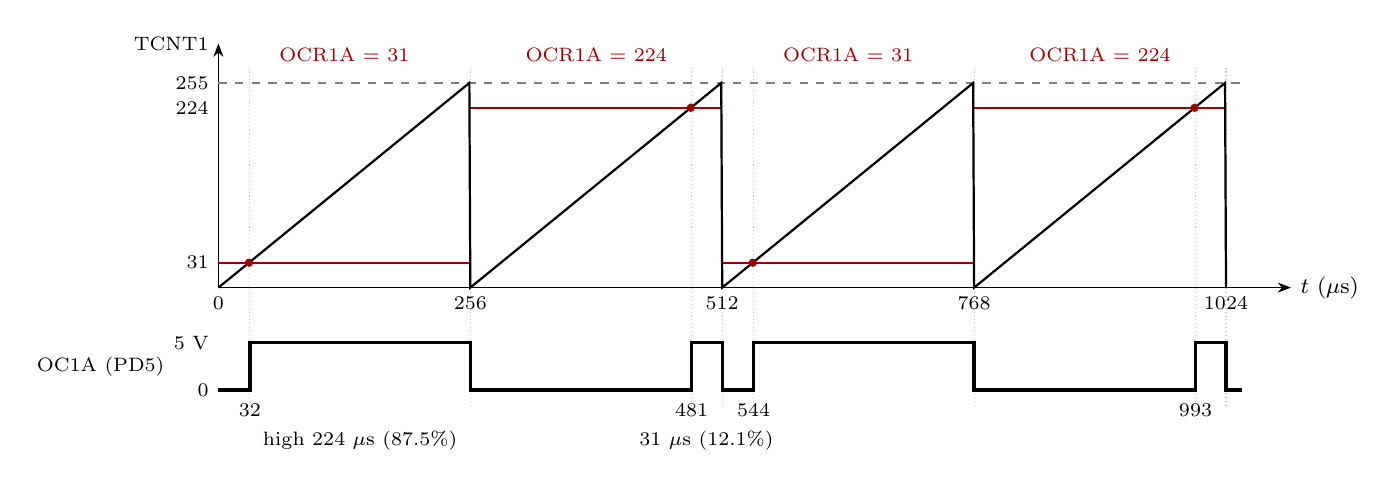
\begin{tikzpicture}[>=Stealth,font=\small,x=0.0125cm,y=1cm]
% 1 unit = 1 us; fast PWM 8-bit (TOP = 255), 256 us per period; inverting: set on match, clear at BOTTOM
% OCR1A per period (double-buffered, updated at TOP): 31, 224, 31, 224
\def\s{0.0102}% 255 counts -> 2.6 cm
\foreach \t in {32,256,481,512,544,768,993,1024} \draw[gray!45,densely dotted] (\t,-1.5) -- (\t,2.8);
\draw[->] (0,0) -- (0,3.1) node[left,font=\scriptsize]{TCNT1};
\draw[->] (0,0) -- (1090,0) node[right,font=\footnotesize]{$t$ ($\mu$s)};
\foreach \v in {31,224,255} \node[anchor=east,font=\scriptsize] at (0,\v*\s) {\v};
\draw[gray,dashed] (0,255*\s) -- (1040,255*\s);
\draw[red!60!black,thick] (0,31*\s) -- (256,31*\s) (512,31*\s) -- (768,31*\s);
\draw[red!60!black,thick] (256,224*\s) -- (512,224*\s) (768,224*\s) -- (1024,224*\s);
\foreach \k/\o in {0/31,1/224,2/31,3/224} \node[font=\scriptsize,red!60!black,anchor=south] at (\k*256+128,2.75) {OCR1A = \o};
\draw[thick] (0,0) \foreach \k in {1,...,4} { -- (\k*256-1,255*\s) -- (\k*256,0) };
\foreach \t/\v in {31/31,480/224,543/31,992/224} \fill[red!60!black] (\t,\v*\s) circle (1.5pt);
\foreach \t in {0,256,512,768,1024} \node[below,font=\scriptsize] at (\t,0) {\t};
\begin{scope}[yshift=-1.3cm]
\node[anchor=east,font=\scriptsize] at (-45,0.3) {OC1A (PD5)};
\node[anchor=east,font=\scriptsize] at (0,0.6) {5 V};
\node[anchor=east,font=\scriptsize] at (0,0) {0};
\draw[very thick] (0,0) -- (32,0) -- (32,0.6) -- (256,0.6) -- (256,0) -- (481,0) -- (481,0.6) -- (512,0.6) -- (512,0) -- (544,0) -- (544,0.6) -- (768,0.6) -- (768,0) -- (993,0) -- (993,0.6) -- (1024,0.6) -- (1024,0) -- (1040,0);
\foreach \t in {32,481,544,993} \node[font=\scriptsize,anchor=north] at (\t,-0.05) {\t};
\node[font=\scriptsize,anchor=north] at (144,-0.4) {high 224 $\mu$s (87.5\%)};
\node[font=\scriptsize,anchor=north] at (496,-0.4) {31 $\mu$s (12.1\%)};
\end{scope}
\end{tikzpicture}
\end{document}
